\documentclass[twocolumn]{article}

\usepackage{amsmath}
\usepackage{graphicx}
\usepackage{url}
\usepackage[round]{natbib}
\usepackage[utf8]{inputenc}
% To make two column figures appear in the correct order
\usepackage{fixltx2e}
% To make annotations on the sides
\usepackage{todonotes}
% To generate dummy text
\usepackage{lipsum}
% Metadata for the generated PDF
\usepackage[pdftex,colorlinks=true]{hyperref}
\hypersetup{
    allcolors=blue,
}


\begin{document}

\title{
    My very cool new paper
}
\author{
    Leonardo Uieda$^{1,2}$,
    Valéria C. F. Barbosa$^{2}$
    \\\\
    {\small
        $^1$Universidade do Estado do Rio de Janeiro, Rio de Janeiro, Brazil.
        e-mail: leouieda@gmail.com
    }
    \\
    {\small
        $^2$Observatório Nacional, Rio de Janeiro, Brazil.
    }
}


\maketitle


\begin{abstract}
    \lipsum[1]
\end{abstract}


%%%%%%%%%%%%%%%%%%%%%%%%%%%%%%%%%%%%%%%%%%%%%%%%%%%%%%%%%%%%%%%%%%%%%%%%%%%%%%%
\section{Introduction}

Cite things using \citet{tikhonov1977} or \citep{tikhonov1977}.

\begin{figure}
    \centering
    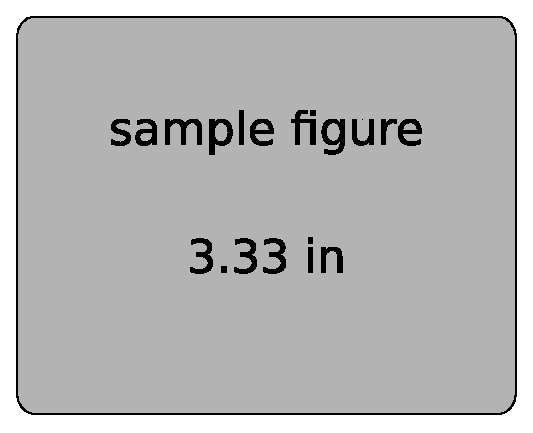
\includegraphics[]{figures/example}
    \caption{
        Example image.
    }
    \label{fig:meh}
\end{figure}


%%%%%%%%%%%%%%%%%%%%%%%%%%%%%%%%%%%%%%%%%%%%%%%%%%%%%%%%%%%%%%%%%%%%%%%%%%%%%%%
\section{Acknowledgments}

We are indebted to the developers and maintainers of the open-source
software without which this work would not have been possible.

%%%%%%%%%%%%%%%%%%%%%%%%%%%%%%%%%%%%%%%%%%%%%%%%%%%%%%%%%%%%%%%%%%%%%%%%%%%%%%%

\bibliographystyle{plainnat}
\bibliography{references}

\end{document}
